% !TeX root = ../main-paper.tex
\section{OCR benchmark}
\label{sec:ocr-xp}

\subsection{Protocol}

Dataset:
- input: image crops for each entry
- expected output: human transcription
- 8765 entries used, \joseph{FIXME number of chars}


Systems
In this benchmark, we consider 3 OCR systems well known for historical document analysis: Pero OCR, Tesseract, and Kraken. 



\subsection{Results and discussion}

\begin{figure}

\subcaptionbox{}[.5\linewidth]{
\begin{tabular}{rlll}
\toprule
 & Pero-OCR  & Tesseract & Kraken \\    
\midrule
CER & 3.78\% & 6.56\% & 15.72\% \\  
\bottomrule
\end{tabular}
\bigskip

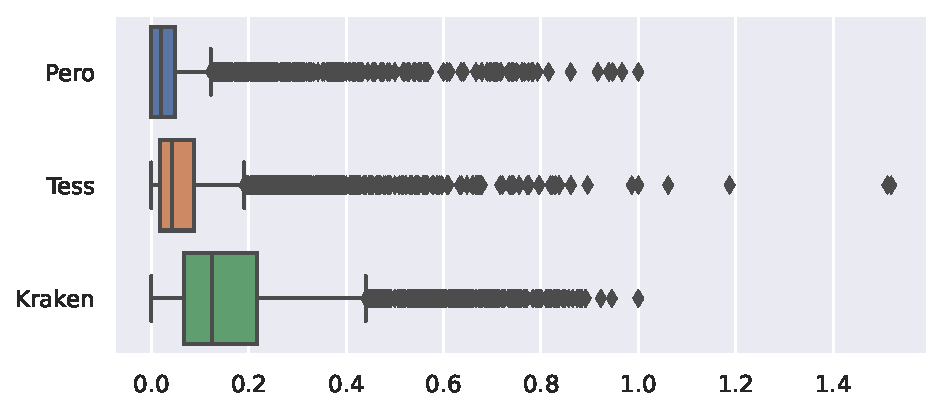
\includegraphics[width=\linewidth]{images/ocr-eval-2.pdf}
\medskip
}
\subcaptionbox{}[.5\linewidth]{
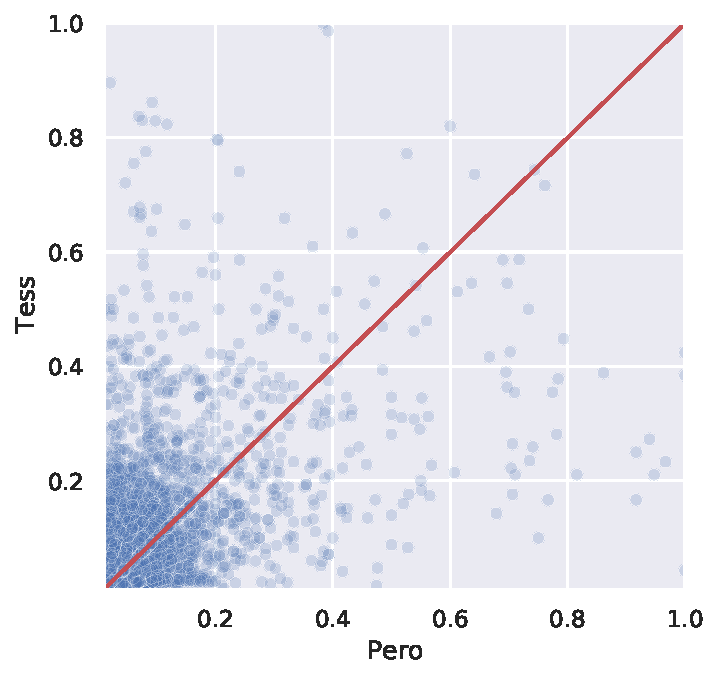
\includegraphics[width=\linewidth]{images/ocr-eval-1.pdf}
}
\caption{Character error rates at entry-level for Pero-OCR, Kraken and Tesseract. (a) Global CER and distribution of the CER per entry. (b)
joint plot of the per-entry error rate showing that Pero-OCR and Tesseract do not fail on the same entries.}  
\label{fig.ocr-results}
\end{figure}

\Cref{fig.ocr-results} compares the performance of the OCR systems on our dataset. We can see Kraken's performance are
not as good as the two first OCR. This is partially due to the fact that the closest available model is for English text
and so it misses French specific symbols. On the over hand, even when using a French model trained on French 19th
documents, performance does not increase (and relaxing the character match rules does not help either). Tesseract and
Pero-OCR are performing better on this dataset ``out-of-the-box''. With no fine-tuning, Pero-OCR gets the best accuracy
with less than 4\% character errors. Many of them are even due to a bad line detection in case of multi-lines entries
and are not related to the OCR system itself. \Cref{fig.ocr-results} (b) shows that errors from the two best OCR are not
committed on the same entries (if so, all points would be on the diagonal line) and that combining the outputs of
Pero-OCR and Tesseract would improve the overall recognition quality. Also, we will not consider Kraken in the following
NER experiments because of its recognition rate is already low and cannot be artificially degraded in a controlled setup.

